%%%%%%%%%%%%%%%%%%%%%%%%%%%%%%%%%%%%%%%%%%%%%%%%%%%%%%%%%%%%%%%%%%%%%%
% UMB-CS110-2015S: Introduction to Computing
% Copyright 2015 Pejman Ghorbanzade <pejman@ghorbanzade.com>
% Creative Commons Attribution-ShareAlike 4.0 International License
% More info: https://github.com/ghorbanzade/UMB-CS110-2015S
%%%%%%%%%%%%%%%%%%%%%%%%%%%%%%%%%%%%%%%%%%%%%%%%%%%%%%%%%%%%%%%%%%%%%%

\def \topDirectory {.}
\def \texDirectory {\topDirectory/src/main/tex}

\documentclass[12pt,letterpaper,twoside]{article}
\usepackage{\texDirectory/template/style/directives}
\usepackage{\texDirectory/template/style/assignment}
%%%%%%%%%%%%%%%%%%%%%%%%%%%%%%%%%%%%%%%%%%%%%%%%%%%%%%%%%%%%%%%%%%%%%%%%%%%%%%
% CS110: Introduction to Computing
% Copyright 2015 Pejman Ghorbanzade <mail@ghorbanzade.com>
% Creative Commons Attribution-ShareAlike 4.0 International License
% https://github.com/ghorbanzade/UMB-CS110-2015S/blob/master/LICENSE
%%%%%%%%%%%%%%%%%%%%%%%%%%%%%%%%%%%%%%%%%%%%%%%%%%%%%%%%%%%%%%%%%%%%%%%%%%%%%%

\course{id}{CS110}
\course{name}{Introduction to Computing}
\course{venue}{Tue/Thu, 5:30 PM - 6:45 PM}
\course{semester}{Spring 2015}
\course{department}{Department of Computer Science}
\course{university}{University of Massachusetts Boston}

\instructor{name}{Pejman Ghorbanzade}
\instructor{title}{}
\instructor{position}{Student Instructor}
\instructor{email}{pejman@cs.umb.edu}
\instructor{phone}{617-287-6419}
\instructor{office}{S-3-124B}
\instructor{office-hours}{Tue/Thu 19:00-20:30}
\instructor{address}{University of Massachusetts Boston, 100 Morrissey Blvd., Boston, MA}


\begin{document}

\doc{title}{Assignment 3}
\doc{date-pub}{Mar 12, 2015 at 5:30 PM}
\doc{date-due}{Apr 02, 2015 at 5:30 PM}
\doc{points}{8}

\prepare{header}

\section*{Question 1}

An alarm clock is simple to use.
You set the alarm, it rings, you snooze and the last two steps are repeated in a \texttt{while(true)} loop! Write a class \texttt{AlarmClock.java} that defines basic functionalities of an alarm clock: setting an alarm, snoozing and dismissing it.

Use your class in a program \texttt{AlarmClockTest.java} where user is asked to set an alarm.
Every ten seconds your program should check if it's time to ring.
After ringing, user is asked either to snooze or dismiss the alarm.
If snoozed, the alarm is set to ring 5 minutes later.
If dismissed, the alarm is deactivated.

\begin{figure}[H]\centering
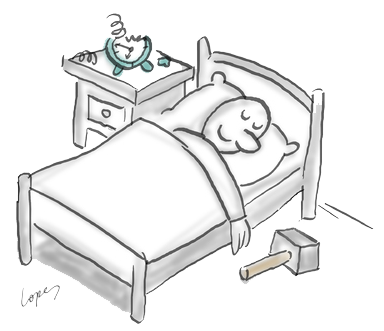
\includegraphics[width=8cm]{\texDirectory/template/images/clock.png}
\end{figure}
\newpage

\section*{Question 2}

Suppose you have \texttt{N} decks of cards, each including thirteen ranks of each of four suits. Our objective is to calculate how many times should we randomly select a card from our collection and turn its face up to get the following (at least):
\begin{enumerate}[itemsep=0mm,label=(\alph*)]
\item one card of each suit
\item one card of each value
\item all thirteen cards of suit hearts in a deck
\item all cards of suit hearts in our collection
\item a standard 52-card deck
\end{enumerate}

\begin{enumerate}
\item Write a program \texttt{DeckShuffle.java} that asks for \texttt{N} and shuffles the decks. Your program should print names of all the shuffled cards, one in each line similar to example given below:
\begin{verbatim}
% java DeckShuffle 5
Four of Hearts
Queen of Clubs
...
\end{verbatim}
\item Write another program \texttt{DeckCollector.java} that takes a shuffled collection as an initialized array and gives number of cards it takes to achieve each above-mentioned objective.
\end{enumerate}

\section*{Question 3}

A group of computer science graduates of University of Massachusetts Boston have recently started a startup company named Beacons Software Solutions.
Currently, they are investing their efforts on developing a Personal Expense Tracking (PET) system.
They are aiming to add a cool feature to PET that allows users to keep track of their bank accounts.
Fortunately, they are short in Java programmers and will surely appreciate your help for this task.

You are asked to write a class \texttt{bankAccount.java} that defines withdrawal, deposit and balance inquiry for a bank account with user-specified name and number.

To check your developed class, write a program \texttt{myAccounts.java} that upon execution, asks a user to initialize his checking and saving accounts by naming them, setting their numbers and declaring their initial balance.
You're program should then prompt user if he would like to withdraw from or deposit into his accounts.
A withdraw transaction is successful only if requested amount is less than available balance.
After each transaction, the user should be asked if he would like to make another transaction.
To simplify the problem, assume each user has two and only two accounts: checking and saving.

As Beacons Software Solutions is aiming to make PET as user-friendly as possible, you are expected to use the \texttt{JOptionPane} class instead of the command-window throughout your \texttt{myAccounts.java} program.

\prepare{footer}

\end{document}
